%% ============================================================
%% 分片 21：原文第 8 节「Electric Eigenbranes」（原文 glshort.tex 起于第 6379 行）
%% 由 tools/harvmac2tex.py 从 arXiv 源码（hep-th/0604151v3）自动生成。
%% 只译英文散文；公式、编号、\label、\cite 一律不改。
%% ============================================================

\section{Electric Eigenbranes}

\label{sec:electricbranes}

In section 第~\ref{sec:loopop}~节, we introduced the topological Wilson and 't
Hooft operators, their action on branes, and the concept of an
electric or magnetic eigenbrane. Our goal in section 第~\ref{sec:wilbranes}~节\
will be to understand explicitly how Wilson operators act on
branes.  Then in section 第~\ref{sec:zerobelectric}~节\ we will use this
information to identify zerobranes as electric eigenbranes.

\subsection{How Wilson Operators Act On Branes}

\label{sec:wilbranes}

As always in this paper, the theory of interest is  twisted ${\cal
N}=4$ super Yang-Mills theory, with gauge group $G$, on a
four-manifold $M$. The fields include a connection $A$ on a
$G$-bundle $E\to M$. We assume $M$ to have a boundary that is
labeled by a brane ${\cal B}$ that respects the topological
symmetry, a condition that of course depends on the parameter
$\Psi$.

Topological Wilson line operators exist if $\Psi=\infty$, which we
achieve by setting $t=i$ with arbitrary gauge coupling $\tau$. Let
$R$ be a representation of $G$.
 A Wilson operator in the representation $R$ and supported
 on a curve ${{\cal S}}$ contributes in the
 path integral a factor % 式 (8.1)
\setcounter{equation}{0}
\begin{equation}\label{eq:yrgy}
W_{{\cal S}}(R)=P\exp\left(-\int_{{\cal S}}(A+i\phi)
 \right).
\end{equation}

 More explicitly, write
$E(R)$ for the bundle associated to $E$ in the representation $R$
of $G$.  The Wilson line operator is the matrix of parallel
transport  along ${{\cal S}}$, in the bundle $E(R)$, with the
connection $\CA=A+i\phi$.  The effect of including this operator
is to add an external charge, in the representation $R$, whose
trajectory in spacetime is ${{\cal S}}$.  If ${{\cal S}}$ is a
closed loop, we take the trace of $W_{{\cal S}}(R)$, and if
instead ${{\cal S}}$ goes off to infinity, we combine $W_{{\cal
S}}(R)$ with initial and final states at the ends of ${{\cal S}}$
so as to make a gauge-invariant expression.

Now we specialize to $M=\Sigma\times C$, so as to be able to
reduce the discussion to a two-dimensional sigma-model with target
$\MH(G,C)$. 
 
 In this  sigma-model, ${\cal
B}$ is represented by a Chan-Paton bundle $U$ (or possibly a more
general sheaf or complex of sheaves \cite{ref103,ref104}) over
the target space $\MH$. $U$ is endowed with a connection $\alpha$.
Since the brane ${\cal B}$ is defined by its Chan-Paton bundle (or
sheaf), a Wilson line operator will have to act on branes by
acting on this bundle or sheaf in some way.

\def\QQ{\eurm Q}

 Let us recall how Chan-Paton bundles enter sigma-models.  We
consider a sigma-model of maps $\Phi:\Sigma\to \MH$, and a brane
${\cal B}$ that is endowed with a Chan-Paton bundle $U\to \MH$
with connection $\alpha$.   The quantum theory is defined by an
integral over the possible maps $\Phi$, along with certain
fermionic variables. One factor in the path integral comes from
the bulk action ${\cmmib I}$ and takes the form
$\exp\left(-\int_\Sigma {{\cmmib I}}\right)$. There also is a
boundary factor that involves parallel transport in the Chan-Paton
bundle. Let $\QQ$ be the part of the boundary of $\Sigma$ that is
labeled by the brane ${\cal B}$, and write $\Phi_\QQ$ for the
restriction of $\Phi$ to $\QQ$. The boundary factor in the path
integral involving $\QQ$ is given by the parallel transport or
holonomy along $\QQ$ of the bundle $\Phi_\QQ^*(U)$:
% 式 (8.2)
\setcounter{equation}{1}
\begin{equation}\label{eq:tomfo}
P\exp\left(-\int_\QQ \left(\Phi_\QQ^*(\alpha)
+\dots\right)\right).
\end{equation}
 If $\QQ$ is a closed circle, we take a
trace of this holonomy, and otherwise this factor combines at the
endpoints of $\QQ$ with other factors, depending on the precise
calculation that one chooses to perform, to make a gauge-invariant
expression. The ellipses in \eqref{eq:tomfo}\ are fermionic corrections to
the connection $\Phi_\QQ^*(\alpha)$ on $\Phi_\QQ^*(U)$.  They are
required by supersymmetry, rather as the shift $A\to {\cal
A}=A+i\phi$ was needed in section 第~\ref{sec:topwil}~节\ to define
supersymmetric Wilson operators.

There is an obvious analogy between the factor \eqref{eq:tomfo}\ by which
Chan-Paton bundles enter in sigma-models and the factor \eqref{eq:yrgy}\ by
which a Wilson line operator influences the underlying
four-dimensional gauge theory.  The analogy is even closer because
to define the action of the Wilson operator on the brane ${\cal
B}$, we must take the limit as ${{\cal S}}$ (or rather its
projection from $\Sigma\times C$ to $\Sigma$) approaches $\QQ$.

To get something precise from this analogy, we begin with the
following observation. When gauge theory on a $G$-bundle $E\to
M=\Sigma\times C$ is described in terms of a map $\Phi:\Sigma\to
\MH$,  the $G$-bundle $E$  can be identified as $(\Phi\times
1)^*({\EUE})$, where ${\EUE}$ is the ``bundle'' part of the
universal Higgs bundle $({\EUE},\hat\varphi)$ over $\MH$, and
$(\Phi\times 1)^*({\EUE})$ is its pullback via the map $\Phi\times
1:\Sigma\times C\to \MH\times C$. This statement just means that,
to the extent that the sigma-model is a good description, for each
point $q\in \Sigma$, the bosonic fields $A,\phi$ of the gauge
theory, when restricted to $q\times C$, are given by the solution
of Hitchin's equations corresponding to the point $\Phi(q)\in
\MH$. This solution is simply, up to a gauge transformation, the
restriction of the universal Higgs bundle $({\EUE},\hat\varphi)$
to $\Phi(q)\times C$.

To interpret the connection ${\cal A}=A+i\phi$ in \eqref{eq:yrgy}\ in terms
of the sigma-model, we note that in general, this connection
involves both $\cA_\Sigma$, the part of  the connection tangent to
$\Sigma$, and $\cA_C$, the part tangent to $C$. Here in the low
energy theory, we can assume that $\cA_C$ obeys Hitchin's
equations, and as long as we avoid singularities in $\MH$, the
fields $\cA_\Sigma$ are massive in the sigma-model. They can
therefore be integrated out in favor of the sigma-model fields
$\cA_C$.  For very large ${\rm Im}\,\tau$,  it is sufficient to
integrate out $\CA_\Sigma$ at the classical level. The part of the
gauge theory action which depends on only $A$ and $\phi$ was
written in \eqref{eq:wingo}. Assuming that $A_C$ and $\phi_C$ satisfy
Hitchin equations and dropping the terms which vanish as the
volume of $C$ goes to zero, we find a quadratic action for
$\cA_\Sigma$. The corresponding equations of motion read
% 式 (8.3)
\setcounter{equation}{2}
\begin{equation}\label{eq:integrout}
\cD_C{}^\dagger \cD_C \cA_\Sigma=\cD_C{}^\dagger
d_\Sigma \cA_C+\dots,
\end{equation}
 where $\cD_C$ is the covariant differential
with respect to the connection $\cA_C$.  The ellipses refer to
terms involving zero modes of the fermions $\psi$, $\tilde\psi$,
etc., of the four-dimensional gauge theory; we will not write
these terms explicitly.   A map $\Phi:\Sigma\to \MH$   determines
$\cA_C$ and hence also $d_\Sigma\cA_C$, and then, assuming we keep
away from singularities of $\MH$, the equation \eqref{eq:integrout}\ has a
unique solution for $\cA_\Sigma$.

So once $\Phi:\Sigma\to \MH$ is given (and assuming that we keep
away from singularities of $\MH$), the connection
$\CA=(\cA_\Sigma,\cA_C)$ is determined.  $\CA$ is, of course, a
connection on the bundle $E=(\Phi\times 1)^*({\EUE})$.
 The connection $\CA$ is actually the pullback by $\Phi\times 1$ of a
connection $\hat\CA$ on  ${\EUE}\to \MH\times C$. In fact, to
define $\hat\CA$, we must specify its components $\CA_{\MH},\CA_C$
tangent to $\MH$ and $C$.  $\CA_C$ is the appropriate solution of
Hitchin's equations, and $\CA_{\MH}$ is defined by generalizing
\eqref{eq:integrout}\ in an obvious way:\footnote{The ellipses in \eqref{eq:integrout}\
involve fermionic zero modes, which represent tangent vectors to
$\MH$ and so have analogs in the case of $\MH\times C$.}
% 式 (8.4)
\setcounter{equation}{3}
\begin{equation}\label{eq:pintegrout}
\cD_C{}^\dagger \cD_C \cA_{\M_H}=\cD_C{}^\dagger
d_{{\eusm M}_H} \cA_C+\dots.
\end{equation}

Now let us specialize to the case that ${{\cal S}}=\gamma\times
p$, with $\gamma$ a curve in $\Sigma$ and $p$ a point in $C$.  We
write ${\EUE}_p(R)$ for the restriction of ${\EUE}(R)$ to
$\MH\times p$. We also write $\Phi_p$ for the restriction to
$\Sigma\times \{p\}\subset \Sigma\times C$ of the map $\Phi\times
1:\Sigma\times C\to \MH\times C$. We can replace the connection
$\CA=A+i\phi$ in \eqref{eq:yrgy}\ by $\Phi_p^*(\hat\CA)$.  Hence the factor
in the path integral that comes from the inclusion of a Wilson
operator on the contour ${{\cal S}}$ in the representation $R$ can
be written as % 式 (8.5)
\setcounter{equation}{4}
\begin{equation}\label{eq:zico}
W_R({{\cal S}})=
P\exp\left(-\int_\gamma\,\Phi_p^*(\hat\CA)\right).
\end{equation}
 In the limit that
$\gamma$ approaches the boundary $\QQ$ of $\Sigma$, this has the
same form as the term that comes anyway from the Chan-Paton bundle
$U$ of the original brane ${\cal B}$:\footnote{The ellipses in \eqref{eq:zomfo}\
represent fermionic terms whose analog in \eqref{eq:zico}\ arises from the
ellipses in \eqref{eq:integrout}, which reflect fermionic contributions to
$\CA_\Sigma$. All these terms are uniquely determined by the
topological symmetry, so we do not need to worry about comparing
them.} % 式 (8.6)
\setcounter{equation}{5}
\begin{equation}\label{eq:zomfo}
P\exp\left(-\int_\QQ (\Phi_\QQ^*(\alpha)
+\dots)\right).
\end{equation}

So we learn how Wilson lines act on branes.  A Wilson line in the
representation $R$ and supported at a point $p\in C$ transforms
the Chan-Paton bundle $U$ of a brane ${\cal B}$ by % 式 (8.7)
\setcounter{equation}{6}
\begin{equation}\label{eq:yuq}
U\to
U\otimes {\EUE}_p(R).
\end{equation}

\par\medskip{\it Transformation Of The $B$-Field}

As we have discussed in section 第~\ref{sec:reviewthis}~节,  ${\EUE}(R)$, and
hence also ${\EUE}_p(R)$, in general does not exist as a vector
bundle. But it always exists as a twisted vector bundle, twisted
by the flat $B$-field $\theta_{R}(\zeta)$, where $\theta_{R}$  is
the character of the center of the gauge group determined by $R$.

The category of branes depends on a choice of $B$-field, a fact
that we exploited in section 第~\ref{sec:comptwop}~节. For a given discrete
electric field ${\bf e}_0$, the background $B$-field in the
sigma-model on $\MH$ is $b_{{\bf e}_0}={\bf e}_0(\zeta)$, where
$\zeta=\xi({\EUE}_{\rm{ad}})$ is the obstruction to existence of a
universal $\bar G$ Higgs bundle. Tensoring with a twisted bundle
that is twisted by $\theta_R(\zeta)$ maps a brane that is twisted
by a flat $B$-field $b$ to a brane that is twisted by
$b+\theta_R(\zeta).$ Therefore, the action of a Wilson line
operator on branes changes the $B$-field, by $b\to
b+\theta_R(\zeta)$.  In other words, it changes the discrete
electric field studied in section 第~\ref{sec:centertop}~节\ by ${\bf e}_0\to
{\bf e}_0+\theta_R$.

We want to understand what this result means for $S$-duality.  So
we write it as a statement about the dual gauge theory, with gauge
group $^ LG$, and a Wilson line $W(^L\negthinspace R)$ determined
by a representation $^L\negthinspace R$.  This Wilson line
transforms the discrete electric field by % 式 (8.8)
\setcounter{equation}{7}
\begin{equation}\label{eq:nuko}
{\bf e}_0\to
{\bf e}_0+\theta(^L\negthinspace R),
\end{equation}
 where, for convenience, we
write $\theta(^L\negthinspace R)$ rather than
$\theta_{^L\negthinspace R}$.

\begin{figure}[htbp]
\centering
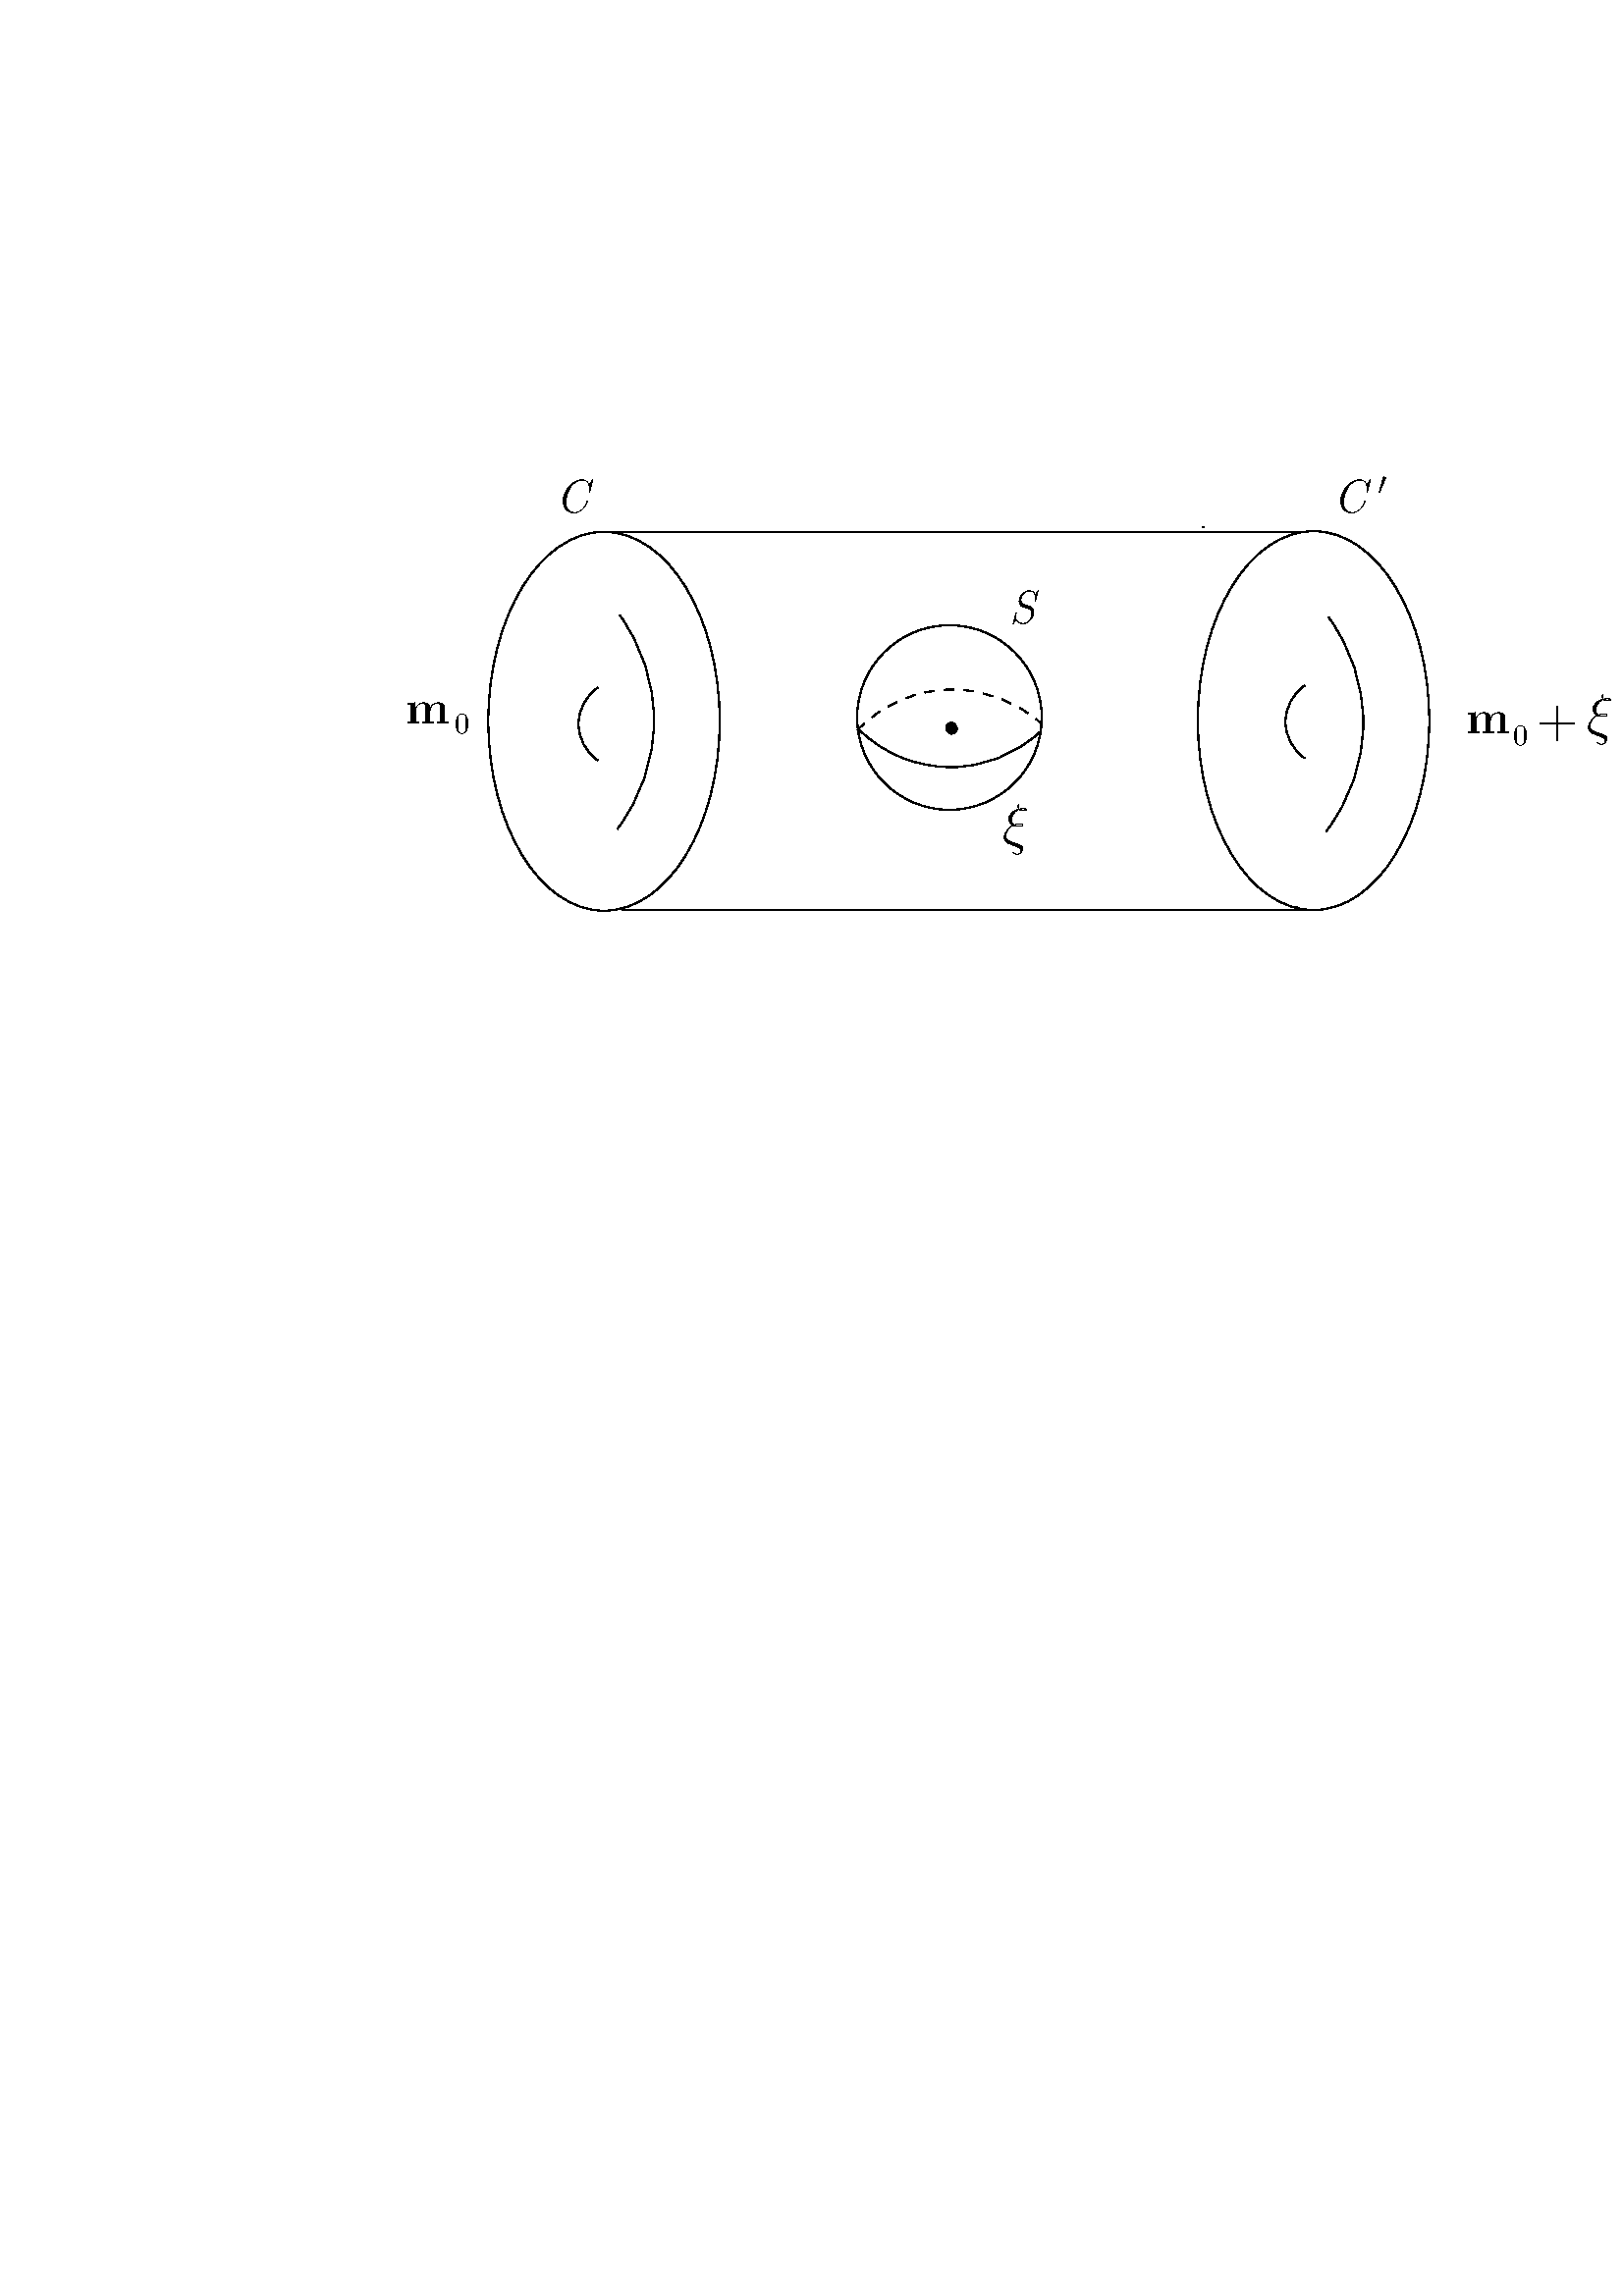
\includegraphics[width=0.75\linewidth]{figures/gla6-1.png}
\caption{Insertion of an 't Hooft operator changes the topology of a $G$-bundle, as shown here. Sketched is a three manifold with boundary components consisting of two Riemann surfaces $C$ and $C'$ and a small two-sphere $S$ enclosing a point at which an 't Hooft operator is inserted. Cobordism invariance of the characteristic class implies that if $\bf{m}_0$ is the characteristic class of the $G$-bundle $E\to C$, then the characteristic class of $E\to C'$ must be ${\bf{m}}_0+\xi$, where $\xi=\xi({}^L\negthinspace R)$ is the characteristic class associated with the 't Hooft operator.（原文 Fig.~11）}
\label{fig:namp}
\end{figure}
 Under $S$-duality, the fact
that a Wilson line operator can change the discrete electric field
${\bf e}_0$ maps to the fact that an 't Hooft line operator can
change the characteristic class ${\bf m}_0\in H^2(C,\pi_1(G))$
which classifies the topology of the $G$-bundle $E\to C$. Indeed,
as we explained in section 第~\ref{sec:tophooft}~节, an 't Hooft operator
$T(^L\negthinspace R)$ is constructed from a $G$-bundle, which we
may call $E(^L\negthinspace R)$, over $S^2\cong \Bbb{CP}^1$.  This
$G$-bundle has a characteristic class $\xi(^L\negthinspace
R)=\xi(E(^L\negthinspace R))$. The action of the 't Hooft operator
on ${\bf m}_0$ is % 式 (8.9)
\setcounter{equation}{8}
\begin{equation}\label{eq:zuko}
{\bf m}_0\to {\bf
m}_0+\xi(^L\negthinspace R).
\end{equation}
 This statement, which is the
$S$-dual of \eqref{eq:nuko}, just comes from the behavior of the
characteristic class under cobordism, as in \namp.

\par\medskip{\it Wilson Operators And Supersymmetry}

Let us see what kind of supersymmetry the operation \eqref{eq:yuq}\
preserves.  For a generic choice of curve ${{\cal S}}\subset
\Sigma\times C$, the supersymmetric Wilson line $W(R,{{\cal S}})$
preserves $B$-type supersymmetry in the complex structure $J$ of
$\MH$ and nothing else. However, if we take ${{\cal
S}}=\gamma\times p$, for $\gamma$ a curve in $\Sigma$ and $p$ a
point in $C$, then the Wilson operator preserves more
supersymetry. In fact, as we showed at the end of section 第~\ref{sec:lineop}~节,
it preserves supersymmetry of type $(B,B,B)$, that is, it
preserves $B$-type supersymmetry in each complex structure.

We can now see explicitly how this is reflected in the action of
the Wilson operator on branes.  For a point $p\in C$, the bundle
${\EUE}_p(R)$ is holomorphic in each of the complex structures on
$\MH$.  (This can be naturally proved using the hyper-Kahler
quotient construction of $\MH$.) So the operation \eqref{eq:yuq}\ preserves
$B$-type supersymmetry for each complex structure.

\subsection{Zerobranes As Electric Eigenbranes}

\label{sec:zerobelectric}

Now we can look for electric eigenbranes.  Consider a Wilson line
$W_q(R)$ in a representation $R$ and at a point $q\in C$.  It maps
a brane ${\cal B}$ with Chan-Paton sheaf $U$ to a brane with
Chan-Paton sheaf $U\otimes {\EUE}_q(R)$.  By definition, ${\cal
B}$ is an electric eigenbrane if $U\otimes {\EUE}_q(R)$ is
isomorphic to $U\otimes V$ for some fixed vector space $V$. The
condition, therefore, is that ${\EUE}_q(R)$ equipped with the
connection $\Phi_q^*(\hat \CA)$ must be holomorphically trivial --
isomorphic to a vector bundle with constant fiber $V$ -- when
restricted to the support of $U$.

Let $x$ be a point in $\MH$, and let ${\cal B}_x$ be a zerobrane
supported at $x$. In other words, ${\cal B}_x$ is a brane whose
Chan-Paton sheaf is a skyscraper sheaf $U_x$ supported at $x$. We
will suppose that $x$ is a smooth point in $\MH$, so that one can
integrate out the fields $A_\Sigma,\phi_\Sigma$ on the classical
level.

Any vector bundle is trivial when restricted to a point, and in
particular the bundle ${\EUE}_q(R)$ is trivial when restricted to
$x\in \MH$.  Its restriction to $x$, which we denote as
${\EUE}_q(R)|_x$, is just a fixed vector space.  So
% 式 (8.10)
\setcounter{equation}{9}
\begin{equation}\label{eq:insto}
U_x\otimes {\EUE}_q(R)=U_x\otimes {\EUE}_q(R)|_x.
\end{equation}

Therefore, ${\cal B}_x$ is an electric eigenbrane, the
``eigenvalue'' of the Wilson loop operator $W_q(R)$ being the
vector space ${\EUE}_q(R)|_x$.

Equivalently, the boundary conditions on the sigma-model fields
corresponding to the zerobrane say that $\cA_C$ is constant up to
a gauge transformation on the boundary of $\Sigma$. By virtue of
\eqref{eq:integrout}, this implies that ${\cal A}_\Sigma$ is trivial on the
boundary of $\Sigma$.

We argued in section 第~\ref{sec:lineop}~节, based on the underlying
four-dimensional topological field theory, that the ``eigenvalue''
of an electric or magnetic eigenbrane must vary with $q\in C$ as
the fiber of a flat bundle over $C$.  Indeed, as $q\in C$ varies,
the space ${\EUE}_q(R)|_x$ does vary as the fiber of a flat vector
bundle. In fact, taking complex structure $J$, the restriction
$({\EUE},\hat\varphi)|_x$ of the universal bundle to $x\times C$
gives a flat $G_{\Bbb{C}}$ bundle ${\EUE}|_x\to C$ (since a
solution of Hitchin's equations corresponds in complex structure
$J$ to a flat $G_{\Bbb{C}}$-bundle). By taking this bundle in the
representation $R$, we get the desired flat bundle whose fiber at
$q\in C$ is ${\EUE}_q(R)|_x$.  We picked here complex structure
$J$ because it is singled out by the underlying topological
supersymmetry.

In describing the zerobrane as an electric eigenbrane, we have
been slightly informal on one key point: the role of the discrete
$B$-field ${\bf e}_0(\zeta)$.  A $B$-field is trivial when
restricted to a point, so as long as one is considering
zerobranes, one can informally ignore the $B$-field, as we have
just done.  However, a more precise way to describe things is as
follows.  For every ${\bf e}_0$, the category of branes contains
an object that is a zerobrane supported at the (smooth) point
$x\in \MH$.  Because the action of a Wilson line operator can
change ${\bf e}_0$, the electric eigenbrane is really a sum of
twisted zerobranes with different ${\bf e}_0$ (all of which are
isomorphic, as the twisting is trivial when restricted to a
point). Dually, since an 't Hooft operator can change ${\bf m}_0$,
the magnetic eigenbranes will be sums of branes supported on
different components of $\MH$, for all possible ${\bf m}_0$.  In
standard approaches to the geometric Langlands program, one says
that the Hecke eigensheaves are supported on the union of all
topological components of $\M(G,C)$.

\par\medskip{\it Relation To The Geometric Langlands Program}

Now we can get at least a glimmering of how all this is related to
the geometric Langlands program.

In the geometric Langlands program, one begins with the  group
$^L\negthinspace G$ and a homomorphism $\vartheta:\pi_1(C)\to{}
^L\negthinspace G_{\Bbb{C}}$. (One requires that this homomorphism
be semistable in a sense explained in section 第~\ref{sec:complexstr}~节.) The
space of such homomorphisms is the Hitchin moduli space
$\MH(^L\negthinspace G,C)$.  So $\vartheta$ defines a point
$x(\vartheta)$ in $\MH(^L\negthinspace G,C)$.

If $\vartheta$ is irreducible, then $x(\vartheta)$ is a smooth
point and a zerobrane ${\cal B}_{x(\vartheta)}$ supported at
$x(\vartheta)$ is an electric eigenbrane.  $S$-duality applied to
this electric eigenbrane will give a magnetic eigenbrane in the
sigma-model of target $\MH(G,C)$.  {}From sections 第~\ref{sec:sdualhitfib}~节\
and 第~\ref{sec:twodimint}~节, we know that the $S$-dual of a zerobrane of
$\MH(^L\negthinspace G,C)$ is a brane in $\MH(G,C)$ whose support
is a fiber ${\CMF}$ of the Hitchin fibration, endowed with a flat
Chan-Paton bundle of rank 1.  We refer to such a brane as a brane
of type ${\CMF}$.

The main claim of the geometric Langlands program is that a
homomorphism $\vartheta:\pi_1(C)\to {}^L\negthinspace G_{\Bbb{C}}$
is associated in a natural way to a sheaf on $\M(G,C)$ that is a
Hecke eigensheaf and also a holonomic ${\cal D}$-module.  Sections
第~\ref{sec:thooftheckeop}~节 -第~\ref{sec:abranes}~节\ of this paper will be devoted to
explaining why a brane of type ${\CMF}$ on $\MH(G,C)$ has the
right properties. In sections 第~\ref{sec:thooftheckeop}~节\ and 第~\ref{sec:bogeqheck}~节, we
relate the 't Hooft operators of quantum gauge theory  to the
Hecke operators of the geometric Langlands program, showing how
our notion of a magnetic eigenbrane is related to the mathematical
concept of a Hecke eigensheaf.  In section 第~\ref{sec:abranes}~节, we argue that
by virtue of the existence of a certain coisotropic $A$-brane on
$\MH(G,C)$, the brane of type ${\CMF}$ is naturally associated to
a module for the differential operators on $\M(G,C)$.
